% Capitolul 10: Recapitulare Completă - Complete Time Series Analysis
% Applying all methods to real data: Bitcoin, Sunspots, Unemployment
% Bachelor program, Bucharest University of Economic Studies

\documentclass[9pt, aspectratio=169, t]{beamer}

% Ensure content fits on slides
\setbeamersize{text margin left=8mm, text margin right=8mm}

%=============================================================================
% THEME AND STYLE CONFIGURATION
%=============================================================================
\usetheme{Madrid}
\usecolortheme{seahorse}

% IDA-Inspired Color Palette
\definecolor{MainBlue}{RGB}{26, 58, 110}
\definecolor{AccentBlue}{RGB}{42, 82, 140}
\definecolor{IDAred}{RGB}{220, 53, 69}
\definecolor{DarkGray}{RGB}{51, 51, 51}
\definecolor{MediumGray}{RGB}{128, 128, 128}
\definecolor{LightGray}{RGB}{248, 248, 248}
\definecolor{VeryLightGray}{RGB}{235, 235, 235}
\definecolor{Crimson}{RGB}{220, 53, 69}
\definecolor{Forest}{RGB}{46, 125, 50}
\definecolor{Amber}{RGB}{181, 133, 63}
\definecolor{Orange}{RGB}{230, 126, 34}
\definecolor{BitcoinOrange}{RGB}{247, 147, 26}

\setbeamercolor{palette primary}{bg=MainBlue, fg=white}
\setbeamercolor{palette secondary}{bg=MainBlue!85, fg=white}
\setbeamercolor{palette tertiary}{bg=MainBlue!70, fg=white}
\setbeamercolor{structure}{fg=MainBlue}
\setbeamercolor{title}{fg=MainBlue}
\setbeamercolor{frametitle}{fg=MainBlue, bg=white}
\setbeamercolor{block title}{bg=MainBlue, fg=white}
\setbeamercolor{block body}{bg=VeryLightGray, fg=DarkGray}
\setbeamercolor{block title alerted}{bg=Crimson, fg=white}
\setbeamercolor{block body alerted}{bg=Crimson!8, fg=DarkGray}
\setbeamercolor{block title example}{bg=Forest, fg=white}
\setbeamercolor{block body example}{bg=Forest!8, fg=DarkGray}
\setbeamercolor{item}{fg=MainBlue}

\setbeamertemplate{navigation symbols}{}

\setbeamertemplate{footline}{
    \leavevmode%
    \hbox{%
        \begin{beamercolorbox}[wd=.333333\paperwidth,ht=2.5ex,dp=1ex,center]{author in head/foot}%
            \usebeamerfont{author in head/foot}\insertshortauthor
        \end{beamercolorbox}%
        \begin{beamercolorbox}[wd=.333333\paperwidth,ht=2.5ex,dp=1ex,center]{title in head/foot}%
            \usebeamerfont{title in head/foot}\insertshorttitle
        \end{beamercolorbox}%
        \begin{beamercolorbox}[wd=.333333\paperwidth,ht=2.5ex,dp=1ex,right]{date in head/foot}%
            \usebeamerfont{date in head/foot}\insertshortdate{}\hspace*{2em}
            \insertframenumber{} / \inserttotalframenumber\hspace*{2ex}
        \end{beamercolorbox}}%
    \vskip0pt%
}

%=============================================================================
% PACKAGES
%=============================================================================
\usepackage[utf8]{inputenc}
\usepackage[T1]{fontenc}
\usepackage{amsmath, amssymb, amsthm}
\usepackage{mathtools}
\usepackage{bm}
\usepackage{tikz}
\usetikzlibrary{arrows.meta, positioning, shapes, calc}
\usepackage{booktabs}
\usepackage{multirow}
\usepackage{array}
\usepackage{graphicx}
\usepackage{hyperref}
\hypersetup{colorlinks=false, pdfborder={0 0 0}}
\graphicspath{{../logos/}{../charts/}}

%=============================================================================
% THEOREM ENVIRONMENTS
%=============================================================================
\theoremstyle{definition}
\setbeamertemplate{theorems}[numbered]
\newtheorem{defn}{Definition}
\newtheorem{thm}{Theorem}
\newtheorem{prop}{Proposition}

%=============================================================================
% CUSTOM COMMANDS
%=============================================================================
\newcommand{\E}{\mathbb{E}}
\newcommand{\Var}{\text{Var}}
\newcommand{\Cov}{\text{Cov}}
\newcommand{\Corr}{\text{Corr}}
\newcommand{\R}{\mathbb{R}}

%=============================================================================
% TITLE INFORMATION
%=============================================================================
\title[Capitolul 10: Recapitulare Completă]{Capitolul 10: Recapitulare Completă}
\subtitle{Bachelor Program, Faculty of Cybernetics, Statistics and Economic Informatics, Bucharest University of Economic Studies}
\author[Prof. Daniel Traian Pele, PhD]{Prof. Daniel Traian Pele, PhD\\[0.2cm]\footnotesize\texttt{danpele@ase.ro}}
\institute{Bucharest University of Economic Studies}
\date{Academic Year 2025--2026}

\begin{document}

%=============================================================================
% TITLE SLIDE
%=============================================================================
\begin{frame}[plain]
    \begin{tikzpicture}[remember picture, overlay]
        \fill[IDAred] (current page.north west) rectangle ([yshift=-0.15cm]current page.north east);
        \node[anchor=north west] at ([xshift=0.5cm, yshift=-0.3cm]current page.north west) {
            \href{https://www.ase.ro}{\includegraphics[height=1.1cm]{ase_logo.png}}
        };
        \node[anchor=north] at ([yshift=-0.3cm]current page.north) {
            \href{https://ai4efin.ase.ro}{\includegraphics[height=1.1cm]{ai4efin_logo.png}}
        };
        \node[anchor=north east] at ([xshift=-0.5cm, yshift=-0.3cm]current page.north east) {
            \href{https://www.digital-finance-msca.com}{\includegraphics[height=1.1cm]{msca_logo.png}}
        };
    \end{tikzpicture}
    \vfill
    \begin{center}
        {\Large\textcolor{MediumGray}{Analiza și Prognoza Seriilor de Timp}}\\[0.3cm]
        {\Huge\textbf{\textcolor{MainBlue}{Capitolul 10: Recapitulare Completă}}}\\[0.5cm]
        {\Large\textcolor{IDAred}{Analiză Completă cu Date Reale}}
    \end{center}
    \vfill

    \begin{tikzpicture}[remember picture, overlay]
        \fill[IDAred] (current page.south west) rectangle ([yshift=0.15cm]current page.south east);
        \node[anchor=south west] at ([xshift=0.5cm, yshift=0.8cm]current page.south west) {
            \href{https://theida.net}{\includegraphics[height=0.9cm]{ida_logo.png}}
        };
        \node[anchor=south] at ([xshift=-3cm, yshift=0.8cm]current page.south) {
            \href{https://blockchain-research-center.com}{\includegraphics[height=0.9cm]{brc_logo.png}}
        };
        \node[anchor=south] at ([yshift=0.8cm]current page.south) {
            \href{https://quantinar.com}{\includegraphics[height=0.9cm]{qr_logo.png}}
        };
        \node[anchor=south] at ([xshift=3cm, yshift=0.8cm]current page.south) {
            \href{https://quantlet.com}{\includegraphics[height=0.9cm]{ql_logo.png}}
        };
        \node[anchor=south east] at ([xshift=-0.5cm, yshift=0.8cm]current page.south east) {
            \href{https://ipe.ro/new}{\includegraphics[height=0.9cm]{acad_logo.png}}
        };
    \end{tikzpicture}
\end{frame}

%=============================================================================
% TABLE OF CONTENTS
%=============================================================================
\begin{frame}{Cuprins}
    \tableofcontents
\end{frame}

%=============================================================================
% SECTION 1: INTRODUCTION
%=============================================================================
\section{Fluxul Complet de Analiză}

\begin{frame}{Prezentare Generală: Metode Studiate}
    \begin{columns}[T]
        \begin{column}{0.48\textwidth}
            \textbf{Metode Clasice}
            \begin{itemize}
                \item \textcolor{MainBlue}{Cap 1:} Fundamentele Seriilor de Timp
                \item \textcolor{MainBlue}{Cap 2:} Modele ARMA
                \item \textcolor{MainBlue}{Cap 3:} Modele ARIMA
                \item \textcolor{MainBlue}{Cap 4:} Modele SARIMA
                \item \textcolor{MainBlue}{Cap 5:} Modele GARCH
            \end{itemize}
        \end{column}
        \begin{column}{0.48\textwidth}
            \textbf{Metode Avansate}
            \begin{itemize}
                \item \textcolor{Forest}{Cap 6:} VAR \& Cauzalitate Granger
                \item \textcolor{Forest}{Cap 7:} Cointegrare \& VECM
                \item \textcolor{Forest}{Cap 8:} Extensii Moderne
                \item \textcolor{Forest}{Cap 9:} Prophet \& TBATS
            \end{itemize}
            \vspace{0.5em}
            \textbf{Astăzi: Aplicăm TOATE pe Date Reale!}
        \end{column}
    \end{columns}
\end{frame}

\begin{frame}{Fluxul Complet de Analiză}
    \begin{center}
        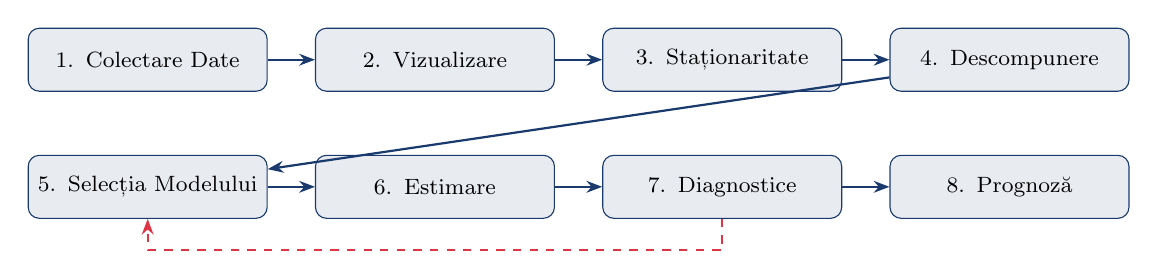
\begin{tikzpicture}[
            node distance=0.6cm,
            box/.style={rectangle, rounded corners, draw=MainBlue, fill=MainBlue!10,
                        text width=2.8cm, minimum height=0.8cm, align=center, font=\footnotesize},
            arrow/.style={-{Stealth[length=2mm]}, thick, MainBlue}
        ]
            % Row 1
            \node[box] (data) {1. Colectare Date};
            \node[box, right=of data] (viz) {2. Vizualizare};
            \node[box, right=of viz] (stat) {3. Staționaritate};
            \node[box, right=of stat] (decomp) {4. Descompunere};

            % Row 2
            \node[box, below=0.8cm of data] (model) {5. Selecția Modelului};
            \node[box, right=of model] (est) {6. Estimare};
            \node[box, right=of est] (diag) {7. Diagnostice};
            \node[box, right=of diag] (forecast) {8. Prognoză};

            % Arrows
            \draw[arrow] (data) -- (viz);
            \draw[arrow] (viz) -- (stat);
            \draw[arrow] (stat) -- (decomp);
            \draw[arrow] (decomp) -- (model);
            \draw[arrow] (model) -- (est);
            \draw[arrow] (est) -- (diag);
            \draw[arrow] (diag) -- (forecast);

            % Feedback loop
            \draw[arrow, dashed, IDAred] (diag.south) -- ++(0,-0.4) -| (model.south);
        \end{tikzpicture}
    \end{center}

    \vspace{0.3cm}
    \begin{alertblock}{Principiu Cheie}
        Diagnosticele pot necesita revenirea la selecția modelului (proces iterativ)
    \end{alertblock}
\end{frame}

\begin{frame}{Seturi de Date Reale pentru Acest Capitol}
    \begin{columns}[T]
        \begin{column}{0.24\textwidth}
            \begin{block}{\textcolor{BitcoinOrange}{Bitcoin}}
                \begin{itemize}
                    \item Zilnic 2019-2024
                    \item Clustering volatilitate
                    \item ARIMA + GARCH
                \end{itemize}
            \end{block}
        \end{column}
        \begin{column}{0.24\textwidth}
            \begin{block}{\textcolor{Orange}{Pete Solare}}
                \begin{itemize}
                    \item Anual 1900-2023
                    \item Ciclu de 11 ani
                    \item Termeni Fourier
                \end{itemize}
            \end{block}
        \end{column}
        \begin{column}{0.24\textwidth}
            \begin{block}{\textcolor{MainBlue}{Șomaj}}
                \begin{itemize}
                    \item Lunar 2010-2023
                    \item Șocul COVID-19
                    \item Prophet
                \end{itemize}
            \end{block}
        \end{column}
        \begin{column}{0.24\textwidth}
            \begin{block}{\textcolor{Forest}{Economic VAR}}
                \begin{itemize}
                    \item Trimestrial 2000-2023
                    \item PIB, Inflație, etc.
                    \item VAR Multivariat
                \end{itemize}
            \end{block}
        \end{column}
    \end{columns}
\end{frame}

%=============================================================================
% TRAIN/VALIDATION/TEST METHODOLOGY
%=============================================================================
\begin{frame}{Metodologie Cheie: Train / Validation / Test Split}
    \begin{center}
        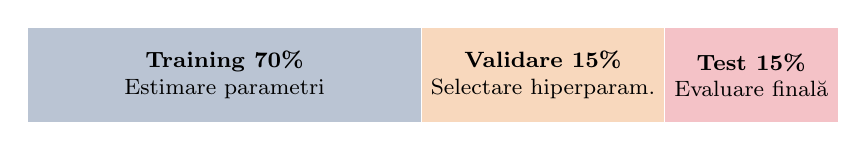
\begin{tikzpicture}[
            box/.style={rectangle, minimum height=1.2cm, align=center, font=\footnotesize},
        ]
            \node[box, fill=MainBlue!30, minimum width=5cm] (train) at (0,0) {\textbf{Training 70\%}\\Estimare parametri};
            \node[box, fill=Orange!30, minimum width=2.2cm, right=-0.01cm of train] (val) {\textbf{Validare 15\%}\\Selectare hiperparam.};
            \node[box, fill=IDAred!30, minimum width=2.2cm, right=-0.01cm of val] (test) {\textbf{Test 15\%}\\Evaluare finală};
        \end{tikzpicture}
    \end{center}

    \vspace{0.3em}
    \begin{columns}[T]
        \begin{column}{0.48\textwidth}
            \textbf{De Ce Contează:}
            \begin{itemize}
                \item \textcolor{MainBlue}{Training}: Estimare parametri model
                \item \textcolor{Orange}{Validare}: Comparare modele, tuning
                \item \textcolor{IDAred}{Test}: Performanță finală nebiasată!
            \end{itemize}
        \end{column}
        \begin{column}{0.48\textwidth}
            \begin{alertblock}{Regulă Critică}
                \textbf{NICIODATĂ} nu priviți datele de test în timpul selecției!

                \vspace{0.2em}
                Pentru serii de timp: \textbf{NICIODATĂ} nu amestecați --- păstrați ordinea temporală.
            \end{alertblock}
        \end{column}
    \end{columns}
\end{frame}

%=============================================================================
% SECTION 2: CASE STUDY 1 - BITCOIN
%=============================================================================
\section{Studiu de Caz 1: Prognoza Volatilității Bitcoin}

\begin{frame}{Bitcoin: Date și Obiectiv}
    \begin{columns}[T]
        \begin{column}{0.55\textwidth}
            \textbf{Date:} Randamente zilnice Bitcoin (2019--2024)
            \begin{itemize}
                \item Sursă: Yahoo Finance (BTC-USD)
                \item 1.826 observații
                \item Randamente = $100 \times \ln(P_t/P_{t-1})$
            \end{itemize}

            \vspace{0.5em}
            \textbf{Obiectiv:} Prognoza \textcolor{IDAred}{volatilității} (nu randamente!)

            \vspace{0.5em}
            \textbf{De ce volatilitatea?}
            \begin{itemize}
                \item Randamentele sunt aproape imprevizibile
                \item Volatilitatea arată persistență puternică
                \item Critică pentru managementul riscului (VaR)
            \end{itemize}
        \end{column}
        \begin{column}{0.43\textwidth}
            \textbf{Împărțire Date:}
            \begin{table}[h]
                \footnotesize
                \begin{tabular}{lcc}
                    \toprule
                    Set & Zile & Perioadă \\
                    \midrule
                    Training & 1.278 & 2019--2022 \\
                    Validare & 274 & 2022--2023 \\
                    Test & 274 & 2023--2024 \\
                    \bottomrule
                \end{tabular}
            \end{table}

            \vspace{0.5em}
            \begin{exampleblock}{Statistici Cheie}
                Randament mediu: 0.12\%/zi \\
                Abatere std: 3.8\%/zi \\
                Kurtoză: 8.2 (cozi groase!)
            \end{exampleblock}
        \end{column}
    \end{columns}
\end{frame}

\begin{frame}{Bitcoin: Selecția Modelului pe Setul de Validare}
    \textbf{Pas 1: Estimare variante GARCH pe Training}

    \textbf{Pas 2: Comparare prognoze volatilitate pe Validare}

    \vspace{0.5em}
    \begin{columns}[T]
        \begin{column}{0.55\textwidth}
            \begin{table}[h]
                \footnotesize
                \begin{tabular}{lccc}
                    \toprule
                    Model & AIC & BIC & \textbf{Val MAE} \\
                    \midrule
                    GARCH(1,1) & 8542 & 8563 & 2.34 \\
                    GARCH(2,1) & 8540 & 8567 & 2.31 \\
                    \textbf{GJR-GARCH(1,1)} & \textbf{8531} & \textbf{8558} & \textbf{2.18} \\
                    EGARCH(1,1) & 8538 & 8565 & 2.25 \\
                    \bottomrule
                \end{tabular}
            \end{table}

            \vspace{0.3em}
            \textcolor{Forest}{$\Rightarrow$ Cel mai bun: GJR-GARCH (captează asimetria)}
        \end{column}
        \begin{column}{0.43\textwidth}
            \textbf{Modelul GJR-GARCH:}
            \[
                \sigma_t^2 = \omega + (\alpha + \gamma I_{t-1}) \varepsilon_{t-1}^2 + \beta \sigma_{t-1}^2
            \]

            \vspace{0.3em}
            Unde $I_{t-1} = 1$ dacă $\varepsilon_{t-1} < 0$

            \vspace{0.5em}
            \begin{alertblock}{Efectul de Levier}
                $\gamma > 0$: Randamentele negative cresc volatilitatea mai mult decât cele pozitive (frică vs lăcomie)
            \end{alertblock}
        \end{column}
    \end{columns}
\end{frame}

\begin{frame}{Bitcoin: Evaluare Finală pe Setul de Test}
    \textbf{Pas 3: Re-estimare GJR-GARCH pe Training+Validare, evaluare pe Test}

    \vspace{0.5em}
    \begin{columns}[T]
        \begin{column}{0.48\textwidth}
            \textbf{Rezultate Set Test:}
            \begin{table}[h]
                \footnotesize
                \begin{tabular}{lc}
                    \toprule
                    Metrică & Valoare \\
                    \midrule
                    Volatilitate MAE & 2.21 \\
                    Volatilitate RMSE & 3.45 \\
                    \bottomrule
                \end{tabular}
            \end{table}

            \vspace{0.5em}
            \textbf{Parametri GJR-GARCH:}
            \begin{itemize}
                \item $\alpha = 0.05$ (efect ARCH)
                \item $\gamma = 0.08$ (efect levier)
                \item $\beta = 0.89$ (persistență)
                \item $\alpha + \gamma/2 + \beta = 0.98$
            \end{itemize}
        \end{column}
        \begin{column}{0.48\textwidth}
            \textbf{Interpretare:}
            \begin{itemize}
                \item Persistență ridicată ($\approx 0.98$)
                \item Efect de levier semnificativ ($\gamma > 0$)
                \item Volatilitatea este previzibilă!
            \end{itemize}

            \vspace{0.5em}
            \begin{exampleblock}{Aplicație Practică}
                \textbf{VaR 1 zi (99\%):}
                \[
                    \text{VaR} = -2.33 \times \hat{\sigma}_{t+1}
                \]
                Dacă $\hat{\sigma} = 4\%$, atunci VaR = $-9.3\%$
            \end{exampleblock}
        \end{column}
    \end{columns}
\end{frame}

\begin{frame}{Bitcoin: Vizualizare Prognoză Volatilitate}
    \begin{center}
        \textbf{Perioada Test: Prognoză vs Volatilitate Realizată}

        \vspace{0.5em}
        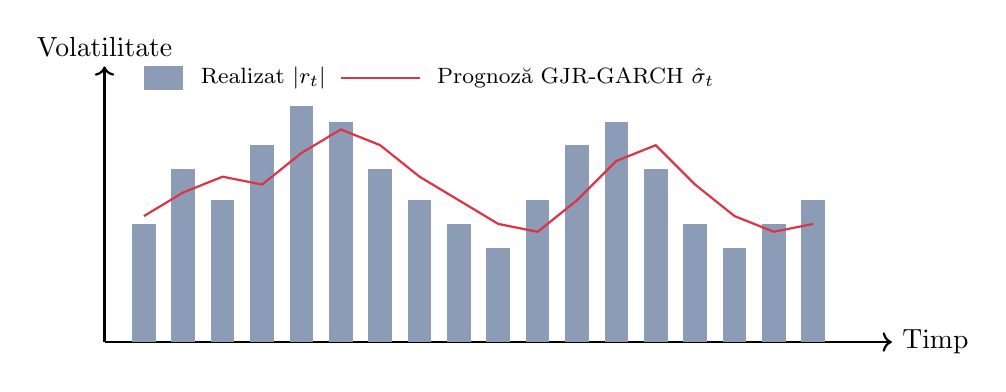
\begin{tikzpicture}
            % Simplified visualization
            \draw[thick, ->] (0,0) -- (10,0) node[right] {Timp};
            \draw[thick, ->] (0,0) -- (0,3.5) node[above] {Volatilitate};

            % Realized volatility (bars)
            \foreach \x/\h in {0.5/1.5, 1/2.2, 1.5/1.8, 2/2.5, 2.5/3, 3/2.8, 3.5/2.2, 4/1.8, 4.5/1.5, 5/1.2, 5.5/1.8, 6/2.5, 6.5/2.8, 7/2.2, 7.5/1.5, 8/1.2, 8.5/1.5, 9/1.8} {
                \fill[MainBlue!50] (\x-0.15,0) rectangle (\x+0.15,\h);
            }

            % Forecast line
            \draw[thick, IDAred] (0.5,1.6) -- (1,1.9) -- (1.5,2.1) -- (2,2.0) -- (2.5,2.4) -- (3,2.7) -- (3.5,2.5) -- (4,2.1) -- (4.5,1.8) -- (5,1.5) -- (5.5,1.4) -- (6,1.8) -- (6.5,2.3) -- (7,2.5) -- (7.5,2.0) -- (8,1.6) -- (8.5,1.4) -- (9,1.5);

            % Legend
            \fill[MainBlue!50] (0.5,3.2) rectangle (1,3.5);
            \node[right, font=\footnotesize] at (1.1,3.35) {Realizat $|r_t|$};
            \draw[thick, IDAred] (3,3.35) -- (4,3.35);
            \node[right, font=\footnotesize] at (4.1,3.35) {Prognoză GJR-GARCH $\hat{\sigma}_t$};
        \end{tikzpicture}
    \end{center}

    \vspace{0.3em}
    \begin{itemize}
        \item Modelul captează clusterele de volatilitate
        \item Prognoza se adaptează la condițiile de piață
        \item Test MAE = 2.21 (bun pentru prognoză zilnică)
    \end{itemize}
\end{frame}

\begin{frame}{Bitcoin: Rezumat}
    \begin{columns}[T]
        \begin{column}{0.48\textwidth}
            \textbf{Metodologie:}
            \begin{enumerate}
                \item Împărțire date: 70/15/15
                \item Comparare variante GARCH pe validare
                \item Selectare cel mai bun model (GJR-GARCH)
                \item Evaluare finală pe test
            \end{enumerate}

            \vspace{0.5em}
            \textbf{Constatare Cheie:}

            Randamentele sunt imprevizibile, dar \textcolor{IDAred}{volatilitatea este previzibilă}!
        \end{column}
        \begin{column}{0.48\textwidth}
            \textbf{Rezultate:}
            \begin{table}[h]
                \footnotesize
                \begin{tabular}{ll}
                    \toprule
                    Cel mai bun model & GJR-GARCH(1,1) \\
                    Validare MAE & 2.18 \\
                    Test MAE & 2.21 \\
                    Insight cheie & Efect de levier \\
                    \bottomrule
                \end{tabular}
            \end{table}

            \vspace{0.5em}
            \begin{exampleblock}{Utilizare Practică}
                \begin{itemize}
                    \item Calcul Value-at-Risk
                    \item Dimensionare poziții
                    \item Evaluare opțiuni
                \end{itemize}
            \end{exampleblock}
        \end{column}
    \end{columns}
\end{frame}

%=============================================================================
% SECTION 3: CASE STUDY 2 - SUNSPOTS
%=============================================================================
\section{Studiu de Caz 2: Prognoza Ciclului Petelor Solare}

\begin{frame}{Pete Solare: Date și Obiectiv}
    \begin{columns}[T]
        \begin{column}{0.55\textwidth}
            \textbf{Date:} Numere anuale pete solare (1900--2023)
            \begin{itemize}
                \item Sursă: statsmodels (dataset Wolfer)
                \item 124 observații anuale
                \item Celebrul ciclu Schwabe de 11 ani
            \end{itemize}

            \vspace{0.5em}
            \textbf{Obiectiv:} Prognoza activității solare

            \vspace{0.5em}
            \textbf{Provocare:}
            \begin{itemize}
                \item SARIMA standard cu $m=11$ este complex
                \item Soluție: Termeni Fourier ca regresori
            \end{itemize}
        \end{column}
        \begin{column}{0.43\textwidth}
            \textbf{Împărțire Date:}
            \begin{table}[h]
                \footnotesize
                \begin{tabular}{lcc}
                    \toprule
                    Set & Ani & Perioadă \\
                    \midrule
                    Training & 87 & 1900--1986 \\
                    Validare & 18 & 1987--2004 \\
                    Test & 19 & 2005--2023 \\
                    \bottomrule
                \end{tabular}
            \end{table}

            \vspace{0.5em}
            \begin{exampleblock}{Statistici Cheie}
                Medie: 76.4 \\
                Abatere std: 56.8 \\
                Perioadă ciclu: $\approx$11 ani
            \end{exampleblock}
        \end{column}
    \end{columns}
\end{frame}

\begin{frame}{Pete Solare: Termeni Fourier pentru Sezonalitate Lungă}
    \textbf{Idee:} Capturăm ciclul de 11 ani cu regresori sinus/cosinus

    \[
        y_t = \mu + \sum_{k=1}^{K} \left[ a_k \sin\left(\frac{2\pi k t}{11}\right) + b_k \cos\left(\frac{2\pi k t}{11}\right) \right] + \text{erori ARMA}
    \]

    \vspace{0.5em}
    \begin{columns}[T]
        \begin{column}{0.48\textwidth}
            \textbf{Câte armonici (K)?}
            \begin{itemize}
                \item K=1: Formă de ciclu de bază
                \item K=2: Vârfuri/văi mai clare
                \item K=3,4: Mai mult detaliu
                \item Prea multe $\Rightarrow$ supraeșantionare
            \end{itemize}

            \vspace{0.3em}
            \textcolor{Forest}{Selectăm K folosind setul de validare!}
        \end{column}
        \begin{column}{0.48\textwidth}
            \begin{alertblock}{De Ce Fourier?}
                \begin{itemize}
                    \item Doar 2K parametri (nu 11)
                    \item Nu e nevoie de diferențiere sezonieră
                    \item Funcționează pentru orice perioadă
                    \item Se combină natural cu ARIMA
                \end{itemize}
            \end{alertblock}
        \end{column}
    \end{columns}
\end{frame}

\begin{frame}{Pete Solare: Selecția Modelului pe Validare}
    \textbf{Model:} ARIMA(2,0,1) + K armonici Fourier

    \vspace{0.5em}
    \begin{columns}[T]
        \begin{column}{0.55\textwidth}
            \begin{table}[h]
                \footnotesize
                \begin{tabular}{lcccc}
                    \toprule
                    K & AIC & BIC & \textbf{Val RMSE} & Val MAE \\
                    \midrule
                    1 & 892 & 905 & 28.4 & 22.1 \\
                    \textbf{2} & \textbf{878} & \textbf{896} & \textbf{24.2} & \textbf{18.9} \\
                    3 & 875 & 898 & 25.1 & 19.5 \\
                    4 & 873 & 901 & 26.8 & 21.2 \\
                    \bottomrule
                \end{tabular}
            \end{table}

            \vspace{0.3em}
            \textcolor{Forest}{$\Rightarrow$ Cel mai bun: K=2 armonici Fourier}

            \vspace{0.3em}
            K=3,4 supraeșantionează: AIC mai mic dar eroare validare mai mare!
        \end{column}
        \begin{column}{0.43\textwidth}
            \textbf{Model Selectat:}

            ARIMA(2,0,1) + 2 perechi Fourier

            \vspace{0.5em}
            \textbf{Parametri:}
            \begin{itemize}
                \item $\phi_1 = 1.35$, $\phi_2 = -0.68$
                \item $\theta_1 = -0.42$
                \item 4 coeficienți Fourier
            \end{itemize}

            \vspace{0.3em}
            Total: 8 parametri
        \end{column}
    \end{columns}
\end{frame}

\begin{frame}{Pete Solare: Evaluare Finală pe Test}
    \textbf{Re-estimare pe Training+Validare, prognoză Test (2005--2023)}

    \vspace{0.5em}
    \begin{columns}[T]
        \begin{column}{0.48\textwidth}
            \textbf{Rezultate Set Test:}
            \begin{table}[h]
                \footnotesize
                \begin{tabular}{lc}
                    \toprule
                    Metrică & Valoare \\
                    \midrule
                    Test RMSE & 26.8 \\
                    Test MAE & 21.4 \\
                    Test MAPE & 42.3\% \\
                    \bottomrule
                \end{tabular}
            \end{table}

            \vspace{0.5em}
            \textbf{Interpretare:}
            \begin{itemize}
                \item Modelul captează timing-ul ciclului
                \item Amplitudinea mai greu de prezis
                \item Intervale de încredere largi
            \end{itemize}
        \end{column}
        \begin{column}{0.48\textwidth}
            \textbf{Prognoză vs Actual (2005--2023):}

            \vspace{0.3em}
            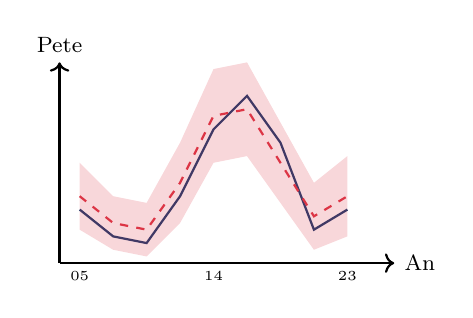
\begin{tikzpicture}[scale=0.85]
                \draw[thick, ->] (0,0) -- (5,0) node[right] {\footnotesize An};
                \draw[thick, ->] (0,0) -- (0,3) node[above] {\footnotesize Pete};

                % Actual values (simplified)
                \draw[thick, MainBlue] (0.3,0.8) -- (0.8,0.4) -- (1.3,0.3) -- (1.8,1.0) -- (2.3,2.0) -- (2.8,2.5) -- (3.3,1.8) -- (3.8,0.5) -- (4.3,0.8);

                % Forecast
                \draw[thick, IDAred, dashed] (0.3,1.0) -- (0.8,0.6) -- (1.3,0.5) -- (1.8,1.2) -- (2.3,2.2) -- (2.8,2.3) -- (3.3,1.5) -- (3.8,0.7) -- (4.3,1.0);

                % Confidence band
                \fill[IDAred, opacity=0.2] (0.3,0.5) -- (0.8,0.2) -- (1.3,0.1) -- (1.8,0.6) -- (2.3,1.5) -- (2.8,1.6) -- (3.3,0.9) -- (3.8,0.2) -- (4.3,0.4) -- (4.3,1.6) -- (3.8,1.2) -- (3.3,2.1) -- (2.8,3.0) -- (2.3,2.9) -- (1.8,1.8) -- (1.3,0.9) -- (0.8,1.0) -- (0.3,1.5) -- cycle;

                % Labels
                \node[font=\tiny] at (0.3,-0.2) {05};
                \node[font=\tiny] at (2.3,-0.2) {14};
                \node[font=\tiny] at (4.3,-0.2) {23};
            \end{tikzpicture}

            \vspace{0.2em}
            {\footnotesize \textcolor{MainBlue}{---} Actual \quad \textcolor{IDAred}{- -} Prognoză \quad \textcolor{IDAred!30}{$\blacksquare$} IC 95\%}
        \end{column}
    \end{columns}
\end{frame}

\begin{frame}{Pete Solare: Rezumat}
    \begin{columns}[T]
        \begin{column}{0.48\textwidth}
            \textbf{Metodologie:}
            \begin{enumerate}
                \item Împărțire: 70/15/15 (ani)
                \item Folosire termeni Fourier pentru ciclu 11 ani
                \item Selectare K pe validare (K=2 optim)
                \item Evaluare finală pe test
            \end{enumerate}

            \vspace{0.5em}
            \textbf{Constatare Cheie:}

            Termenii Fourier captează eficient tiparele sezoniere lungi fără a pierde date prin diferențiere.
        \end{column}
        \begin{column}{0.48\textwidth}
            \textbf{Rezultate:}
            \begin{table}[h]
                \footnotesize
                \begin{tabular}{ll}
                    \toprule
                    Cel mai bun model & ARIMA(2,0,1)+Fourier(2) \\
                    Validare RMSE & 24.2 \\
                    Test RMSE & 26.8 \\
                    Insight cheie & K=2 optim \\
                    \bottomrule
                \end{tabular}
            \end{table}

            \vspace{0.5em}
            \begin{alertblock}{Lecție}
                Pentru perioade sezoniere lungi:
                \begin{itemize}
                    \item Fourier > SARIMA
                    \item Selectați K prin validare încrucișată
                \end{itemize}
            \end{alertblock}
        \end{column}
    \end{columns}
\end{frame}

%=============================================================================
% SECTION 4: CASE STUDY 3 - UNEMPLOYMENT
%=============================================================================
\section{Studiu de Caz 3: Prognoza Șomajului SUA}

\begin{frame}{Șomaj: Date și Provocare}
    \begin{columns}[T]
        \begin{column}{0.55\textwidth}
            \textbf{Date:} Rata Șomajului SUA (2010--2023)
            \begin{itemize}
                \item Sursă: FRED (UNRATE)
                \item 168 observații lunare
                \item Ruptură structurală majoră: COVID-19
            \end{itemize}

            \vspace{0.5em}
            \textbf{Provocarea:}
            \begin{itemize}
                \item Aprilie 2020: 3.5\% $\rightarrow$ 14.7\% (+10.3 pp)
                \item Cea mai mare creștere lunară din istorie
                \item ARIMA tradițional nu face față
            \end{itemize}

            \vspace{0.5em}
            \textbf{Soluție:} Prophet cu detecție changepoints
        \end{column}
        \begin{column}{0.43\textwidth}
            \textbf{Împărțire Date:}
            \begin{table}[h]
                \footnotesize
                \begin{tabular}{lcc}
                    \toprule
                    Set & Luni & Perioadă \\
                    \midrule
                    Training & 118 & 2010--2019 \\
                    Validare & 25 & 2020--2021 \\
                    Test & 25 & 2022--2023 \\
                    \bottomrule
                \end{tabular}
            \end{table}

            \vspace{0.3em}
            \begin{alertblock}{Notă}
                Validarea include șocul COVID --- testează adaptabilitatea modelului
            \end{alertblock}
        \end{column}
    \end{columns}
\end{frame}

\begin{frame}{Prophet: Detecția Changepoints}
    \textbf{Parametru Cheie:} \texttt{changepoint\_prior\_scale}

    \vspace{0.5em}
    \begin{columns}[T]
        \begin{column}{0.48\textwidth}
            \textbf{Ce controlează:}
            \begin{itemize}
                \item Flexibilitatea schimbărilor de trend
                \item Mic (0.01): Trend neted, rigid
                \item Mare (0.5): Multe changepoints permise
            \end{itemize}

            \vspace{0.5em}
            \textbf{Pentru date COVID:}
            \begin{itemize}
                \item Nevoie de flexibilitate pentru salt brusc
                \item Dar nu prea mult (supraeșantionare)
                \item \textcolor{Forest}{Selectăm prin validare!}
            \end{itemize}
        \end{column}
        \begin{column}{0.48\textwidth}
            \textbf{Modelul Prophet:}
            \[
                y(t) = g(t) + s(t) + h(t) + \epsilon_t
            \]

            Unde:
            \begin{itemize}
                \item $g(t)$: Trend liniar pe bucăți
                \item $s(t)$: Sezonalitate (Fourier)
                \item $h(t)$: Efecte sărbători
                \item Changepoints: Unde panta $g(t)$ se schimbă
            \end{itemize}
        \end{column}
    \end{columns}
\end{frame}

\begin{frame}{Șomaj: Selecția Modelului pe Validare}
    \textbf{Testare valori diferite \texttt{changepoint\_prior\_scale}:}

    \vspace{0.5em}
    \begin{columns}[T]
        \begin{column}{0.55\textwidth}
            \begin{table}[h]
                \footnotesize
                \begin{tabular}{lccc}
                    \toprule
                    Scale & Changepoints & \textbf{Val RMSE} & Val MAE \\
                    \midrule
                    0.01 & 2 & 2.85 & 2.31 \\
                    0.05 & 4 & 1.92 & 1.54 \\
                    \textbf{0.10} & \textbf{5} & \textbf{1.24} & \textbf{0.98} \\
                    0.30 & 8 & 1.31 & 1.05 \\
                    0.50 & 12 & 1.48 & 1.19 \\
                    \bottomrule
                \end{tabular}
            \end{table}

            \vspace{0.3em}
            \textcolor{Forest}{$\Rightarrow$ Cel mai bun: scale = 0.10}

            \vspace{0.3em}
            Changepoints detectate:
            \begin{itemize}
                \item Martie 2020 (început COVID)
                \item Aprilie 2020 (vârf)
                \item Iunie 2020 (început recuperare)
            \end{itemize}
        \end{column}
        \begin{column}{0.43\textwidth}
            \textbf{De ce 0.10 câștigă:}
            \begin{itemize}
                \item Destul de flexibil pentru COVID
                \item Nu supraeșantionează zgomotul
                \item Echilibrează bias/varianță
            \end{itemize}

            \vspace{0.5em}
            \begin{exampleblock}{Insight Cheie}
                scale = 0.50 a detectat 12 changepoints --- prea multe!

                Modelul urmărea zgomotul pe termen scurt.
            \end{exampleblock}
        \end{column}
    \end{columns}
\end{frame}

\begin{frame}{Șomaj: Evaluare Finală pe Test}
    \textbf{Re-estimare Prophet (scale=0.10) pe Training+Validare, prognoză Test (2022--2023)}

    \vspace{0.5em}
    \begin{columns}[T]
        \begin{column}{0.48\textwidth}
            \textbf{Rezultate Set Test:}
            \begin{table}[h]
                \footnotesize
                \begin{tabular}{lc}
                    \toprule
                    Metrică & Valoare \\
                    \midrule
                    Test RMSE & 0.42 \\
                    Test MAE & 0.35 \\
                    Test MAPE & 9.8\% \\
                    \bottomrule
                \end{tabular}
            \end{table}

            \vspace{0.5em}
            \textbf{Comparație cu ARIMA:}
            \begin{table}[h]
                \footnotesize
                \begin{tabular}{lcc}
                    \toprule
                    Model & Test RMSE \\
                    \midrule
                    ARIMA(2,1,2) & 0.89 \\
                    \textbf{Prophet} & \textbf{0.42} \\
                    \bottomrule
                \end{tabular}
            \end{table}
        \end{column}
        \begin{column}{0.48\textwidth}
            \textbf{Vizualizare Prognoză (2022--2023):}

            \vspace{0.3em}
            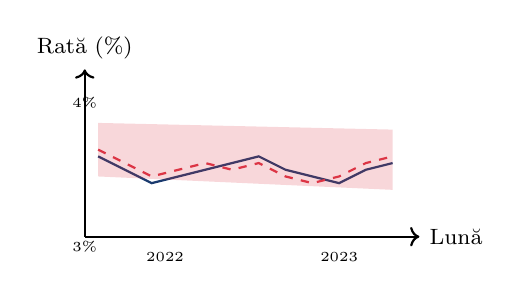
\begin{tikzpicture}[scale=0.85]
                \draw[thick, ->] (0,0) -- (5,0) node[right] {\footnotesize Lună};
                \draw[thick, ->] (0,0) -- (0,2.5) node[above] {\footnotesize Rată (\%)};

                % Axis labels
                \node[font=\tiny] at (0,-0.15) {3\%};
                \node[font=\tiny] at (0,2) {4\%};

                % Actual values
                \draw[thick, MainBlue] (0.2,1.2) -- (0.6,1.0) -- (1,0.8) -- (1.4,0.9) -- (1.8,1.0) -- (2.2,1.1) -- (2.6,1.2) -- (3,1.0) -- (3.4,0.9) -- (3.8,0.8) -- (4.2,1.0) -- (4.6,1.1);

                % Forecast
                \draw[thick, IDAred, dashed] (0.2,1.3) -- (0.6,1.1) -- (1,0.9) -- (1.4,1.0) -- (1.8,1.1) -- (2.2,1.0) -- (2.6,1.1) -- (3,0.9) -- (3.4,0.8) -- (3.8,0.9) -- (4.2,1.1) -- (4.6,1.2);

                % CI band
                \fill[IDAred, opacity=0.2] (0.2,0.9) -- (4.6,0.7) -- (4.6,1.6) -- (0.2,1.7) -- cycle;

                % Year labels
                \node[font=\tiny] at (1.2,-0.3) {2022};
                \node[font=\tiny] at (3.8,-0.3) {2023};
            \end{tikzpicture}

            \vspace{0.2em}
            {\footnotesize \textcolor{MainBlue}{---} Actual \quad \textcolor{IDAred}{- -} Prophet}
        \end{column}
    \end{columns}
\end{frame}

\begin{frame}{Șomaj: Rezumat}
    \begin{columns}[T]
        \begin{column}{0.48\textwidth}
            \textbf{Metodologie:}
            \begin{enumerate}
                \item Împărțire: 70/15/15 (luni)
                \item Tuning \texttt{changepoint\_prior\_scale}
                \item Selectare scale optim pe validare
                \item Evaluare finală pe test
            \end{enumerate}

            \vspace{0.5em}
            \textbf{Constatare Cheie:}

            Prophet gestionează rupturile structurale mai bine decât ARIMA prin detecția automată a changepoints.
        \end{column}
        \begin{column}{0.48\textwidth}
            \textbf{Rezultate:}
            \begin{table}[h]
                \footnotesize
                \begin{tabular}{ll}
                    \toprule
                    Cel mai bun model & Prophet (scale=0.10) \\
                    Validare RMSE & 1.24 \\
                    Test RMSE & 0.42 \\
                    vs ARIMA & 53\% mai bun \\
                    \bottomrule
                \end{tabular}
            \end{table}

            \vspace{0.5em}
            \begin{alertblock}{Lecție}
                Pentru date cu rupturi structurale:
                \begin{itemize}
                    \item Prophet > ARIMA tradițional
                    \item Ajustați flexibilitatea changepoints
                \end{itemize}
            \end{alertblock}
        \end{column}
    \end{columns}
\end{frame}

%=============================================================================
% SECTION 5: CASE STUDY 4 - VAR MULTIVARIATE
%=============================================================================
\section{Studiu de Caz 4: Prognoza Multivariată VAR}

\begin{frame}{VAR: Date și Obiectiv}
    \begin{columns}[T]
        \begin{column}{0.55\textwidth}
            \textbf{Date:} Indicatori Economici SUA (2001--2023)
            \begin{itemize}
                \item Sursă: FRED
                \item 92 observații trimestriale
                \item 4 variabile (PIB, Șomaj, Inflație, Rata Fed)
            \end{itemize}

            \vspace{0.5em}
            \textbf{Obiectiv:} Prognoză conjunctă + analiza relațiilor

            \vspace{0.5em}
            \textbf{De ce VAR?}
            \begin{itemize}
                \item Variabilele se influențează reciproc
                \item Bucle de feedback (PIB $\leftrightarrow$ Șomaj)
                \item Transmisia politicii (Fed $\rightarrow$ Economie)
            \end{itemize}
        \end{column}
        \begin{column}{0.43\textwidth}
            \textbf{Împărțire Date:}
            \begin{table}[h]
                \footnotesize
                \begin{tabular}{lcc}
                    \toprule
                    Set & Trimestre & Perioadă \\
                    \midrule
                    Training & 64 & 2001--2016 \\
                    Validare & 14 & 2017--2020 \\
                    Test & 14 & 2021--2023 \\
                    \bottomrule
                \end{tabular}
            \end{table}

            \vspace{0.3em}
            \textbf{Variabile:}
            \begin{itemize}
                \item Creștere PIB (YoY \%)
                \item Șomaj (\%)
                \item Inflație (CPI YoY \%)
                \item Rata Fed Funds (\%)
            \end{itemize}
        \end{column}
    \end{columns}
\end{frame}

\begin{frame}{VAR: Selecția Ordinului Lag pe Validare}
    \textbf{Model VAR(p):}
    $\mathbf{y}_t = \mathbf{c} + \mathbf{A}_1 \mathbf{y}_{t-1} + \cdots + \mathbf{A}_p \mathbf{y}_{t-p} + \boldsymbol{\varepsilon}_t$

    \vspace{0.5em}
    \begin{columns}[T]
        \begin{column}{0.55\textwidth}
            \textbf{Selectare ordine lag p:}
            \begin{table}[h]
                \footnotesize
                \begin{tabular}{lcccc}
                    \toprule
                    Lag & AIC & BIC & \textbf{Val RMSE} \\
                    \midrule
                    1 & 12.4 & 13.1 & 1.85 \\
                    \textbf{2} & \textbf{11.8} & \textbf{13.0} & \textbf{1.42} \\
                    3 & 11.6 & 13.4 & 1.51 \\
                    4 & 11.5 & 13.8 & 1.68 \\
                    \bottomrule
                \end{tabular}
            \end{table}

            \vspace{0.3em}
            \textcolor{Forest}{$\Rightarrow$ Cel mai bun: VAR(2)}

            \vspace{0.3em}
            Lag-uri mai mari: AIC mai mic dar eroare validare mai mare (supraeșantionare)
        \end{column}
        \begin{column}{0.43\textwidth}
            \textbf{Parametri VAR(2):}
            \begin{itemize}
                \item 4 variabile $\times$ 2 lag-uri = 8 coef per ecuație
                \item + 4 intercepte
                \item Total: 36 parametri
            \end{itemize}

            \vspace{0.5em}
            \begin{alertblock}{BIC vs AIC}
                BIC selectează p=2 (mai simplu)

                AIC selectează p=3 (complex)

                Validarea confirmă BIC!
            \end{alertblock}
        \end{column}
    \end{columns}
\end{frame}

\begin{frame}{VAR: Rezultate Cauzalitate Granger}
    \textbf{Testare relații predictive (pe date Training):}

    \vspace{0.5em}
    \begin{columns}[T]
        \begin{column}{0.55\textwidth}
            \begin{table}[h]
                \footnotesize
                \begin{tabular}{lccc}
                    \toprule
                    Cauză $\rightarrow$ Efect & F-stat & p-value & Sig. \\
                    \midrule
                    PIB $\rightarrow$ Șomaj & 4.82 & 0.012 & ** \\
                    Șomaj $\rightarrow$ PIB & 1.45 & 0.243 & \\
                    Inflație $\rightarrow$ Rata Fed & 6.21 & 0.004 & ** \\
                    Rata Fed $\rightarrow$ Inflație & 2.88 & 0.065 & * \\
                    PIB $\rightarrow$ Inflație & 3.12 & 0.052 & * \\
                    Fed $\rightarrow$ Șomaj & 2.15 & 0.127 & \\
                    \bottomrule
                \end{tabular}
            \end{table}

            {\footnotesize ** p<0.05, * p<0.10}
        \end{column}
        \begin{column}{0.43\textwidth}
            \textbf{Interpretare:}
            \begin{itemize}
                \item PIB conduce șomajul (Legea Okun confirmată)
                \item Inflația conduce politica Fed (Regula Taylor)
                \item Bidirecțional: Fed $\leftrightarrow$ Inflație
            \end{itemize}

            \vspace{0.3em}
            \begin{exampleblock}{Atenție}
                Cauzalitate Granger = predictivă, nu cauzalitate reală!
            \end{exampleblock}
        \end{column}
    \end{columns}
\end{frame}

\begin{frame}{VAR: Evaluare Finală pe Test}
    \textbf{Re-estimare VAR(2) pe Training+Validare, prognoză Test (2021--2023)}

    \vspace{0.5em}
    \begin{columns}[T]
        \begin{column}{0.55\textwidth}
            \textbf{Rezultate Test (per variabilă):}
            \begin{table}[h]
                \footnotesize
                \begin{tabular}{lccc}
                    \toprule
                    Variabilă & RMSE & MAE & vs AR(2) \\
                    \midrule
                    Creștere PIB & 1.82 & 1.45 & -18\% \\
                    Șomaj & 0.58 & 0.44 & -25\% \\
                    Inflație & 1.24 & 0.98 & -12\% \\
                    Rata Fed & 0.89 & 0.72 & -31\% \\
                    \midrule
                    \textbf{Medie} & \textbf{1.13} & \textbf{0.90} & \textbf{-22\%} \\
                    \bottomrule
                \end{tabular}
            \end{table}

            \vspace{0.3em}
            VAR(2) bate AR(2) univariat cu 22\% în medie!
        \end{column}
        \begin{column}{0.43\textwidth}
            \textbf{De ce VAR câștigă:}
            \begin{itemize}
                \item Folosește informația inter-variabile
                \item PIB ajută la predicția șomajului
                \item Inflația ajută la predicția Fed
            \end{itemize}

            \vspace{0.5em}
            \begin{exampleblock}{Cea Mai Mare Îmbunătățire}
                Rata Fed: -31\% RMSE

                De ce? Inflația este un indicator puternic pentru politica Fed.
            \end{exampleblock}
        \end{column}
    \end{columns}
\end{frame}

\begin{frame}{VAR: Analiză Funcții Răspuns la Impuls}
    \textbf{Cum afectează un șoc de 1\% PIB celelalte variabile?}

    \vspace{0.3em}
    \begin{center}
        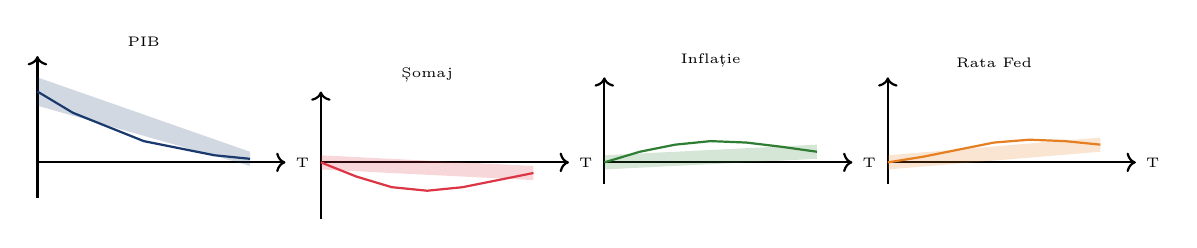
\begin{tikzpicture}[scale=0.9]
            % GDP response
            \begin{scope}[shift={(0,0)}]
                \draw[thick, ->] (0,0) -- (3.5,0) node[right] {\tiny T};
                \draw[thick, ->] (0,-0.5) -- (0,1.5);
                \node[font=\tiny, above] at (1.5,1.5) {PIB};
                \draw[thick, MainBlue] (0,1) -- (0.5,0.7) -- (1,0.5) -- (1.5,0.3) -- (2,0.2) -- (2.5,0.1) -- (3,0.05);
                \fill[MainBlue, opacity=0.2] (0,1.2) -- (3,0.15) -- (3,-0.05) -- (0,0.8) -- cycle;
            \end{scope}

            % Unemployment response
            \begin{scope}[shift={(4,0)}]
                \draw[thick, ->] (0,0) -- (3.5,0) node[right] {\tiny T};
                \draw[thick, ->] (0,-0.8) -- (0,1);
                \node[font=\tiny, above] at (1.5,1) {Șomaj};
                \draw[thick, IDAred] (0,0) -- (0.5,-0.2) -- (1,-0.35) -- (1.5,-0.4) -- (2,-0.35) -- (2.5,-0.25) -- (3,-0.15);
                \fill[IDAred, opacity=0.2] (0,0.1) -- (3,-0.05) -- (3,-0.25) -- (0,-0.1) -- cycle;
            \end{scope}

            % Inflation response
            \begin{scope}[shift={(8,0)}]
                \draw[thick, ->] (0,0) -- (3.5,0) node[right] {\tiny T};
                \draw[thick, ->] (0,-0.3) -- (0,1.2);
                \node[font=\tiny, above] at (1.5,1.2) {Inflație};
                \draw[thick, Forest] (0,0) -- (0.5,0.15) -- (1,0.25) -- (1.5,0.3) -- (2,0.28) -- (2.5,0.22) -- (3,0.15);
                \fill[Forest, opacity=0.2] (0,0.1) -- (3,0.25) -- (3,0.05) -- (0,-0.1) -- cycle;
            \end{scope}

            % Fed response
            \begin{scope}[shift={(12,0)}]
                \draw[thick, ->] (0,0) -- (3.5,0) node[right] {\tiny T};
                \draw[thick, ->] (0,-0.3) -- (0,1.2);
                \node[font=\tiny, above] at (1.5,1.2) {Rata Fed};
                \draw[thick, Orange] (0,0) -- (0.5,0.08) -- (1,0.18) -- (1.5,0.28) -- (2,0.32) -- (2.5,0.3) -- (3,0.25);
                \fill[Orange, opacity=0.2] (0,0.1) -- (3,0.35) -- (3,0.15) -- (0,-0.1) -- cycle;
            \end{scope}
        \end{tikzpicture}
    \end{center}

    \vspace{0.3em}
    \textbf{Interpretare (din IRF):}
    \begin{itemize}
        \item Șoc PIB $\Rightarrow$ Șomajul scade 4-6 trimestre (Legea Okun)
        \item Șoc PIB $\Rightarrow$ Inflația crește, vârf la T3-T4 (cerere-push)
        \item Șoc PIB $\Rightarrow$ Rata Fed crește cu întârziere (răspuns politică)
    \end{itemize}
\end{frame}

\begin{frame}{VAR: Rezumat}
    \begin{columns}[T]
        \begin{column}{0.48\textwidth}
            \textbf{Metodologie:}
            \begin{enumerate}
                \item Împărțire: 70/15/15 (trimestre)
                \item Selectare ordine lag pe validare (p=2)
                \item Testare cauzalitate Granger
                \item Analiză IRF
                \item Prognoză finală pe test
            \end{enumerate}

            \vspace{0.5em}
            \textbf{Constatare Cheie:}

            VAR captează interdependențele economice pe care modelele univariate le pierd.
        \end{column}
        \begin{column}{0.48\textwidth}
            \textbf{Rezultate:}
            \begin{table}[h]
                \footnotesize
                \begin{tabular}{ll}
                    \toprule
                    Cel mai bun model & VAR(2) \\
                    Validare RMSE & 1.42 \\
                    Test RMSE & 1.13 \\
                    vs Univariat & 22\% mai bun \\
                    \bottomrule
                \end{tabular}
            \end{table}

            \vspace{0.5em}
            \begin{exampleblock}{Aplicații}
                \begin{itemize}
                    \item Prognoză macroeconomică
                    \item Analiză impact politici
                    \item Risc portofoliu (multi-activ)
                \end{itemize}
            \end{exampleblock}
        \end{column}
    \end{columns}
\end{frame}

%=============================================================================
% SECTION 6: MODEL SELECTION GUIDE
%=============================================================================
\section{Selecția Modelului: Ghid Practic}

\begin{frame}{Cadrul de Decizie}
    \begin{center}
        \includegraphics[width=0.90\textwidth, height=0.70\textheight, keepaspectratio]{ch10_model_selection_flowchart.pdf}
    \end{center}
\end{frame}

\begin{frame}{Rezumat Selecție Model}
    \begin{table}[h]
        \footnotesize
        \centering
        \begin{tabular}{p{2.5cm}p{3.5cm}p{3.5cm}p{3cm}}
            \toprule
            \textbf{Tip Date} & \textbf{Caracteristici} & \textbf{Model Recomandat} & \textbf{Alternative} \\
            \midrule
            Randamente financiare & Fără trend, clustering vol. & ARIMA-GARCH & EGARCH, GJR \\
            \addlinespace
            Sezonalitate simplă & Trend + o perioadă sezon. & SARIMA & ETS, Prophet \\
            \addlinespace
            Cicluri lungi & Pete solare, cicluri business & AR + Fourier, TBATS & Metode spectrale \\
            \addlinespace
            Rupturi structurale & COVID, schimbări regim & Prophet & ARIMA intervenție \\
            \addlinespace
            Serii multiple & Interdependențe & VAR, VECM & Modele factoriale \\
            \bottomrule
        \end{tabular}
    \end{table}
\end{frame}

\begin{frame}{Metrici de Evaluare a Prognozei}
    \begin{columns}[T]
        \begin{column}{0.48\textwidth}
            \textbf{Metrici pentru Prognoze Punctuale:}

            \vspace{0.3em}
            \textbf{RMSE} (Root Mean Square Error):
            \[
                \sqrt{\frac{1}{n}\sum_{i=1}^{n}(y_i - \hat{y}_i)^2}
            \]

            \textbf{MAE} (Mean Absolute Error):
            \[
                \frac{1}{n}\sum_{i=1}^{n}|y_i - \hat{y}_i|
            \]

            \textbf{MAPE} (Mean Absolute \% Error):
            \[
                \frac{100}{n}\sum_{i=1}^{n}\left|\frac{y_i - \hat{y}_i}{y_i}\right|
            \]
        \end{column}
        \begin{column}{0.48\textwidth}
            \textbf{Când să Folosim Fiecare:}
            \begin{itemize}
                \item \textbf{RMSE}: Penalizează erorile mari
                \item \textbf{MAE}: Robust la outlieri
                \item \textbf{MAPE}: Independent de scală
            \end{itemize}

            \vspace{0.5em}
            \begin{alertblock}{Validare Încrucișată}
                Folosiți întotdeauna CV pentru serii de timp:
                \begin{itemize}
                    \item Fereastră rulantă
                    \item Fereastră expandabilă
                    \item Nu amestecați niciodată!
                \end{itemize}
            \end{alertblock}
        \end{column}
    \end{columns}
\end{frame}

%=============================================================================
% SECTION 6: SUMMARY
%=============================================================================
\section{Rezumat și Concluzii Cheie}

\begin{frame}{Rezumatul Cursului: Setul Complet de Instrumente}
    \begin{columns}[T]
        \begin{column}{0.48\textwidth}
            \textbf{Înțelegerea Datelor}
            \begin{itemize}
                \item Vizualizare mai întâi!
                \item Testați staționaritatea (ADF, KPSS)
                \item Identificați tipare sezoniere
                \item Verificați rupturi structurale
            \end{itemize}

            \vspace{0.5em}
            \textbf{Modele Clasice}
            \begin{itemize}
                \item ARIMA: Date nesezoniere
                \item SARIMA: Sezonalitate simplă
                \item GARCH: Modelarea volatilității
            \end{itemize}
        \end{column}
        \begin{column}{0.48\textwidth}
            \textbf{Abordări Moderne}
            \begin{itemize}
                \item Prophet: Interpretabil, gestionează rupturi
                \item TBATS: Sezonalități multiple/lungi
                \item VAR/VECM: Serii de timp multiple
            \end{itemize}

            \vspace{0.5em}
            \textbf{Cele Mai Bune Practici}
            \begin{itemize}
                \item Verificați întotdeauna diagnosticele
                \item Folosiți validare încrucișată
                \item Comparați modele multiple
                \item Cunoașterea domeniului contează!
            \end{itemize}
        \end{column}
    \end{columns}
\end{frame}

\begin{frame}{Recomandări Finale}
    \begin{enumerate}
        \item \textbf{Începeți Simplu}: Începeți cu vizualizare și statistici de bază
        \item \textbf{Testați Ipotezele}: Staționaritate, normalitate, independență
        \item \textbf{Iterați}: Model $\rightarrow$ Diagnostice $\rightarrow$ Îmbunătățire
        \item \textbf{Comparați}: Nu vă bazați niciodată pe un singur model
        \item \textbf{Validați}: Testarea out-of-sample este esențială
        \item \textbf{Comunicați}: Vizualizări și interpretări clare
    \end{enumerate}

    \vspace{0.5em}
    \begin{exampleblock}{Amintiți-vă}
        ``Toate modelele sunt greșite, dar unele sunt utile.'' --- George Box

        \vspace{0.3em}
        Scopul nu este predicția perfectă, ci perspective utile și prognoze rezonabile.
    \end{exampleblock}
\end{frame}

\begin{frame}{Întrebări?}
    \begin{center}
        \Large\textcolor{MainBlue}{Întrebări?}

        \vspace{1cm}

        \normalsize
        \textbf{Pași Următori:}
        \begin{itemize}
            \item Exersați cu notebook-ul Jupyter
            \item Aplicați aceste metode pe propriile date
            \item Comparați diferite modele pe același set de date
        \end{itemize}

        \vspace{0.5cm}

        Materiale Curs: \texttt{github.com/danpele/Time-Series-Analysis}
    \end{center}
\end{frame}

\end{document}
